\documentclass[11pt]{beamer}
\usetheme{Antibes}
\usepackage{ragged2e}
\defbeamertemplate{description item}{align left}{\insertdescriptionitem\hfill}
\usepackage {tikz}
\usetikzlibrary{positioning}
\definecolor {processblue}{cmyk}{0.96,0,0,0}
\title{FTech Training}
\subtitle{Using Beamer}
\author{Luc Nguyen}
\institute{HUST}
\date{\today}
\usetheme{Boadilla}
\begin{document} % auto-compile by Ctrl + S
	\begin{frame}
		\frametitle{\textbf{CONVOLUTIONAL NEURAL NETWORK}}
		\framesubtitle{OUTLINE}
		\begin{itemize}
			\item \textbf{Basic concepts}
			\item Convolutional Neural Network History
			\item Convolutional Neural Network Architectures
			% \item Some techniques/methods
			\item Applications  
		\end{itemize}
	\end{frame}
	\begin{frame}
		\frametitle{\textbf{CONVOLUTIONAL NEURAL NETWORK}}
		\framesubtitle{Basic concepts}
		\setbeamertemplate{description item}[align left]
		\centering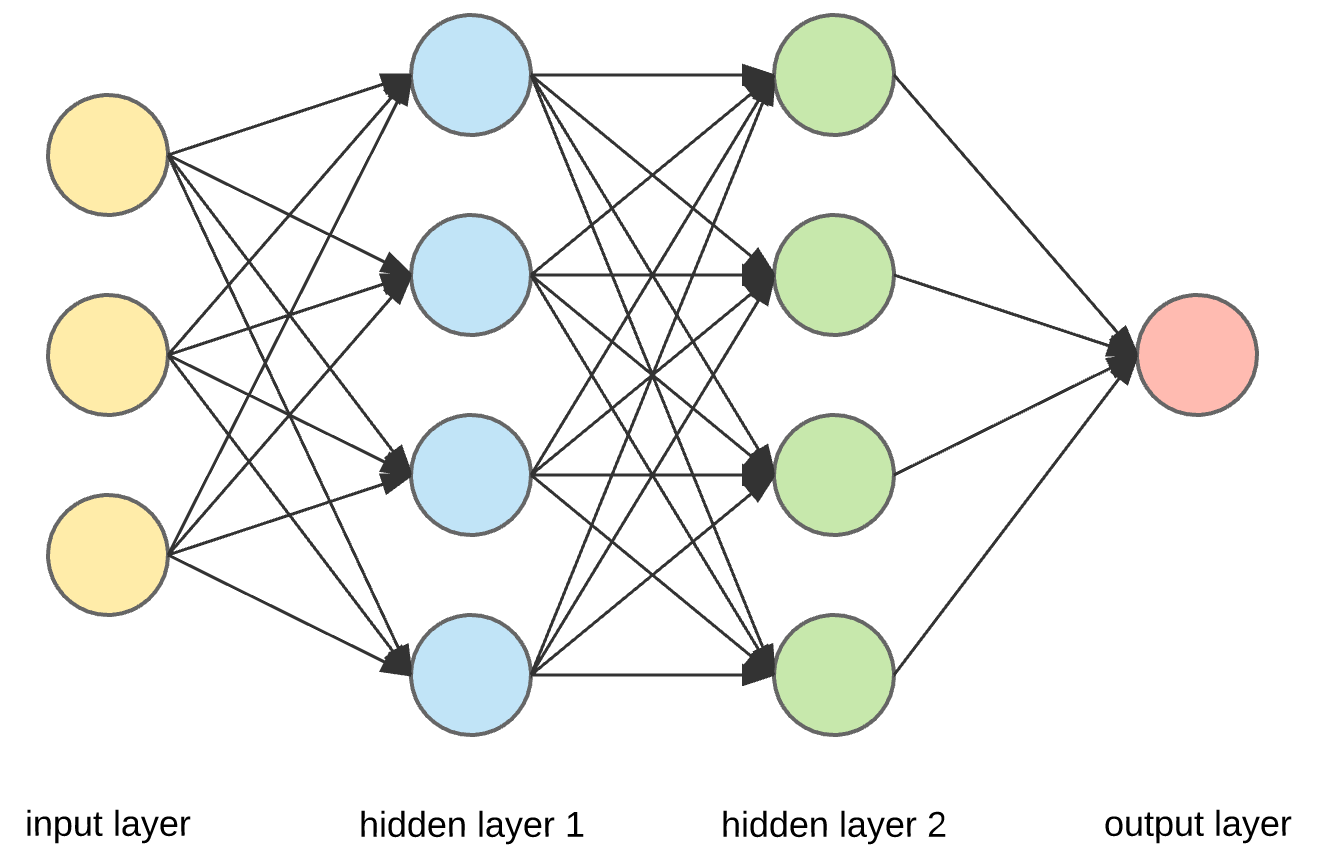
\includegraphics[scale=0.1]{CNN_Visualize.png}
		\begin{description}
			\item[Neural network]A network or a ciucuit of neurons
			\item[Artificial neural networks(ANN)]computing systems insipred by biological neural network that constitute animal brain
			\item[Node] Also called a neuron or Perceptron, is a computational unit that has one or more weighted input connections
			\item[Layers] Sets of neurons
			\item[Convolutional neural network] Artificial neural networks where the connections between layers appear to be somewhat arbitrary
		\end{description}
	\end{frame}
	\begin{frame}
		\frametitle{\textbf{CONVOLUTIONAL NEURAL NETWORK}}
		\framesubtitle{Convolutional Neural Network History}
		\begin{itemize}
			\item 
		\end{itemize}
		
	\end{frame}
	% \begin{frame}
		% 	\frametitle{\textbf{CONVOLUTIONAL NEURAL NETWORK}}
		% 	\framesubtitle{Convolutional Neural Network Layers}
		% 	\begin{center}
	% 		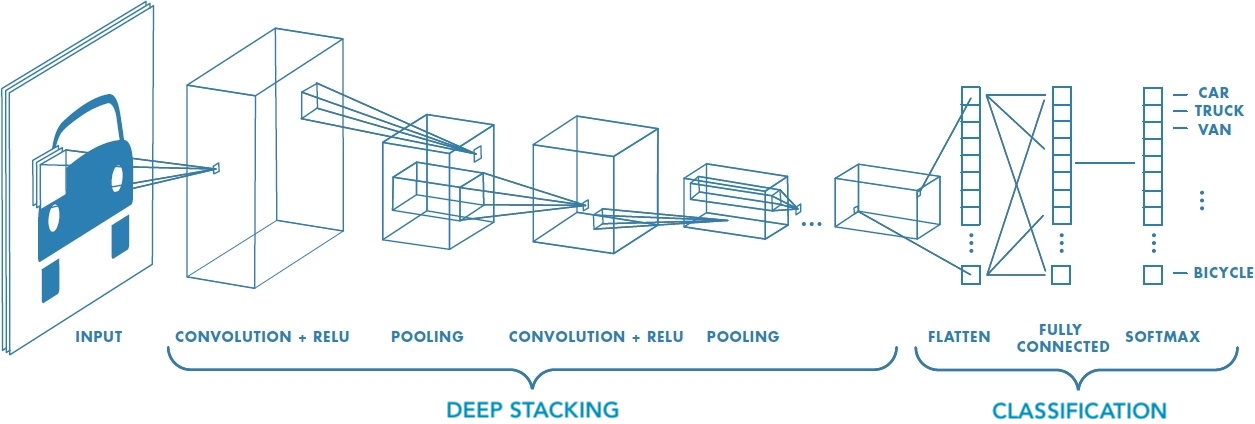
\includegraphics[scale=0.2]{CNN_Layers.png}
	% 	\end{center}
	% 	% \centering\includegraphics[scale=0.2]{ConvNet.gif}
	% 	The Convolutional layer is the core building block of a Convolutional Network that does most of the computational heavy lifting.
	% 	\begin{itemize}
	% 		\item s
	% 	\end{itemize}
	% \end{frame}

	% a high pixels picture => zoom in =>
	% dont much care about each pixel
	% => CNN
	
\end{document}